\chapter{Engine source structure}
\label{app:source}

Table~\ref{tab:app-source} lists the modules of the engine with their size
in lines. The shared modules sit at the top of the package and each part has
its own sub-package with the modules described in
Table~\ref{tab:part-modules}.

\begin{longtable}{>{\raggedright\arraybackslash}p{0.36\textwidth}r>{\raggedright\arraybackslash}p{0.46\textwidth}}
\caption{Engine modules}\label{tab:app-source}\\
\toprule
\textbf{Module} & \textbf{Lines} & \textbf{Purpose}\\
\midrule
\endfirsthead
\toprule
\textbf{Module} & \textbf{Lines} & \textbf{Purpose}\\
\midrule
\endhead
\code{checks.py} & 117 & Common check record and part report\\
\code{loads.py} & 126 & Padeye loads, including the oblique sling\\
\code{working.py} & 59 & Working steps for checks\\
\code{hydro.py} & 127 & Hess-Smith panel method and cavitation number\\
\code{fea/mesh.py} & 129 & Gmsh meshing of STEP solids\\
\code{fea/solver.py} & 356 & P2 elasticity, traction loads, tensor nodal stress, 6-DOF balance, direct and multigrid solvers\\
\code{fea\_study.py} & 128 & Three-mesh study, convergence and force balance\\
\code{optimize/nelder\_mead.py} & 89 & Bounded Nelder-Mead search\\
\code{rules/asme\_bth1.py} & 193 & ASME BTH-1 rule set\\
\code{rules/aisc360.py} & 66 & AISC 360-16 ASD rule set\\
\code{rules/iacs\_s10.py} & 87 & IACS UR S10 rule set, astern factors and bearing limits\\
\code{data/} & 174 & Loader for materials, shackles, pipes and plate stock; shackle side-load table\\
\code{parts/registry.py} & 137 & List of parts for the server and application\\
\code{parts/padeye/} & 2,166 & Padeye job, geometry, checks, working, sizing, CAD, DXF, FEA, Fusion model\\
\code{parts/bracket/} & 1,467 & Bracket job, pipe span, bracket flexibility, geometry, checks, sizing, CAD, FEA\\
\code{parts/stabilizer/} & 1,129 & Fin job, loads ahead and astern, bearings, geometry, checks, sizing, CAD, FEA\\
\code{report\_pdf.py} & 998 & PDF calculation package for the padeye, and shared page layout\\
\code{report\_parts.py} & 582 & PDF sections for the bracket and the fin, with their Fusion cross-check\\
\code{projects.py} & 188 & Projects, runs and their folders\\
\code{runlog.py} & 76 & Engineering log\\
\code{verification.py} & 269 & Benchmark suite\\
\code{server.py} & 539 & Local web server\\
\code{fusion\_link.py} & 181 & Fusion job queue\\
\code{fusion\_sheet.py} & 163 & Fusion cross-check sheet\\
\bottomrule
\end{longtable}

\chapter{Automated tests}
\label{app:tests}

Table~\ref{tab:app-tests} lists the test files. Some tests run once for each
of several inputs, which is why the CAD file holds 54 tests. All 181 tests
pass.

\begin{table}[H]
\centering
\caption{Automated tests}
\label{tab:app-tests}
\small
\begin{tabularx}{\textwidth}{lrX}
\toprule
\textbf{File} & \textbf{Tests} & \textbf{What is tested}\\
\midrule
\code{test\_padeye\_hand\_calc.py} & 7 & Every BTH-1 quantity against the hand calculation\\
\code{test\_padeye\_behaviour.py} & 19 & Each check responds correctly when one input changes\\
\code{test\_padeye\_cad.py} & 54 & Solid volume against the formula for random designs; STEP export and re-import\\
\code{test\_padeye\_fea.py} & 6 & Padeye finite element model, force balance, convergence, fast assembly\\
\code{test\_padeye\_sizing.py} & 9 & Sizing results, targets, rounding, stock and shackle choices\\
\code{test\_fea\_benchmarks.py} & 2 & Cantilever and plate with a hole\\
\code{test\_fea\_vv\_regressions.py} & 7 & 6-DOF equilibrium, zero-moment axial side load, cheek-step exclusion, tensor nodal stress, Frocht--Hill pin-loaded lug $K_{tn}$ benchmark, Fusion unit guards and cross-check sheet\\
\code{test\_bracket.py} & 9 & Bracket loads, pipe span, checks, sizing and FEA\\
\code{test\_stabilizer.py} & 11 & Fin loads, panel method, checks, sizing and stock FEA\\
\code{test\_transparency.py} & 9 & Working results equal check values; engineering log and design records\\
\code{test\_projects\_pipeline.py} & 7 & Projects, runs and output files\\
\code{test\_server.py} & 8 & Server routes for the padeye\\
\code{test\_server\_parts.py} & 6 & Server routes for the bracket and the fin\\
\code{test\_fusion\_link.py} & 7 & Fusion job queue, pickup and expiry, material record, refused reactions\\
\code{test\_advanced\_settings.py} & 20 & Oblique sling and shackle side loading, bracket flexibility, fin astern condition and bearings, by hand\\
\midrule
\textbf{Total} & \textbf{181} & \\
\bottomrule
\end{tabularx}
\end{table}

\chapter{Case-study job descriptions}
\label{app:jobs}

The engine stores each job as a JSON file. Listing~\ref{lst:padeye-job}
shows the job of the padeye case study as the engine saved it. The bracket and
fin jobs have the same form with their own fields, listed in
Table~\ref{tab:cases}.

\begin{lstlisting}[language={}, caption={Job description of the padeye case study}, label={lst:padeye-job}]
{
  "part": "padeye",
  "lift": {
    "lifted_mass_kg": 5000.0,
    "lift_points": 2,
    "sling_angle_deg": 60.0,
    "dynamic_factor": 1.0,
    "points_carrying": null,
    "side_load_fraction": 0.05
  },
  "material_id": "S355",
  "plate_thicknesses_mm": [6, 8, 10, 12, 15, 20, 25, 30, 40, 50],
  "allow_cheek_plates": true,
  "rule_set_id": "asme-bth-1",
  "design_category": "B",
  "service_class": 0,
  "fill_shackle_jaw": true,
  "electrode_strength_mpa": 482.0
}
\end{lstlisting}

\chapter{Selected source code}
\label{app:code}

Listing~\ref{lst:nelder-mead} shows the main loop of the bounded Nelder-Mead
search described in Section~\ref{sec:sizing}. Every trial point is clipped to
the unit box, and values are cached so that a repeated point is not evaluated
twice.

\begin{lstlisting}[language=Python, caption={Main loop of the bounded Nelder-Mead search, from \code{optimize/nelder\_mead.py}}, label={lst:nelder-mead}]
for iterations in range(1, max_iter + 1):
    order = sorted(range(n + 1), key=lambda i: values[i])
    simplex = [simplex[i] for i in order]
    values = [values[i] for i in order]
    if abs(values[-1] - values[0]) <= tolerance * (abs(values[0]) + 1e-12):
        spread = max(max(abs(a - b) for a, b in zip(v, simplex[0])) for v in simplex[1:])
        if spread < 1e-4:
            break

    centroid = [sum(v[d] for v in simplex[:-1]) / n for d in range(n)]
    worst = simplex[-1]
    reflected = _clip([c + (c - w) for c, w in zip(centroid, worst)])
    fr = f(reflected)
    if values[0] <= fr < values[-2]:
        simplex[-1], values[-1] = reflected, fr
        continue
    if fr < values[0]:
        expanded = _clip([c + 2.0 * (r - c) for c, r in zip(centroid, reflected)])
        fe = f(expanded)
        simplex[-1], values[-1] = (expanded, fe) if fe < fr else (reflected, fr)
        continue
    contracted = _clip([c + 0.5 * (w - c) for c, w in zip(centroid, worst)])
    fc = f(contracted)
    if fc < values[-1]:
        simplex[-1], values[-1] = contracted, fc
        continue
    best = simplex[0]
    for i in range(1, n + 1):
        simplex[i] = _clip([b + 0.5 * (v - b) for b, v in zip(best, simplex[i])])
        values[i] = f(simplex[i])
\end{lstlisting}

Listing~\ref{lst:check-record} shows the common check record of
Section~\ref{sec:check-model}.

\begin{lstlisting}[language=Python, caption={Common check record, from \code{checks.py}}, label={lst:check-record}]
@dataclass(frozen=True)
class CheckResult:
    id: str
    title: str
    demand: float
    capacity: float
    unit: str
    source: str
    explanation: str
    basis: Basis = "rule"            # "rule" or "practice"
    severity: Severity = "required"  # "required" or "advice"
    category: Category = "strength"  # "strength", "fit", "stiffness", "span"
    details: dict[str, float] = field(default_factory=dict)
    working: tuple = ()

    @property
    def utilization(self) -> float:
        if self.capacity <= 0:
            return float("inf")
        return self.demand / self.capacity

    @property
    def passed(self) -> bool:
        return bool(self.utilization <= 1.0 + 1e-12)
\end{lstlisting}

\chapter{Using \NEMO{}}
\label{app:user-steps}

The steps below summarise the user guide that comes with the tool.

\begin{enumerate}
    \item Double-click \code{Install NEMO.bat}. This is needed once and
    requires an internet connection.
    \item Double-click the NEMO shortcut on the desktop, or
    \code{Start NEMO.bat}. The application opens in the browser.
    \item Press \emph{New design} and choose the part (Figure~\ref{fig:app-new}).
    \item Fill in the job description. The 3D preview updates as values
    change. Tick the plate thicknesses the workshop holds.
    \item Check the assumptions and change any that do not fit the job.
    \item Press \emph{Find designs} and follow the run on the live screen.
    \item Compare the three designs, open the checks to see their working,
    and download the PDF package and the STEP and DXF files.
    \item Optionally, send a padeye to Fusion to edit it there and check the
    edited design in \NEMO{}.
\end{enumerate}

\begin{figure}[H]
\centering
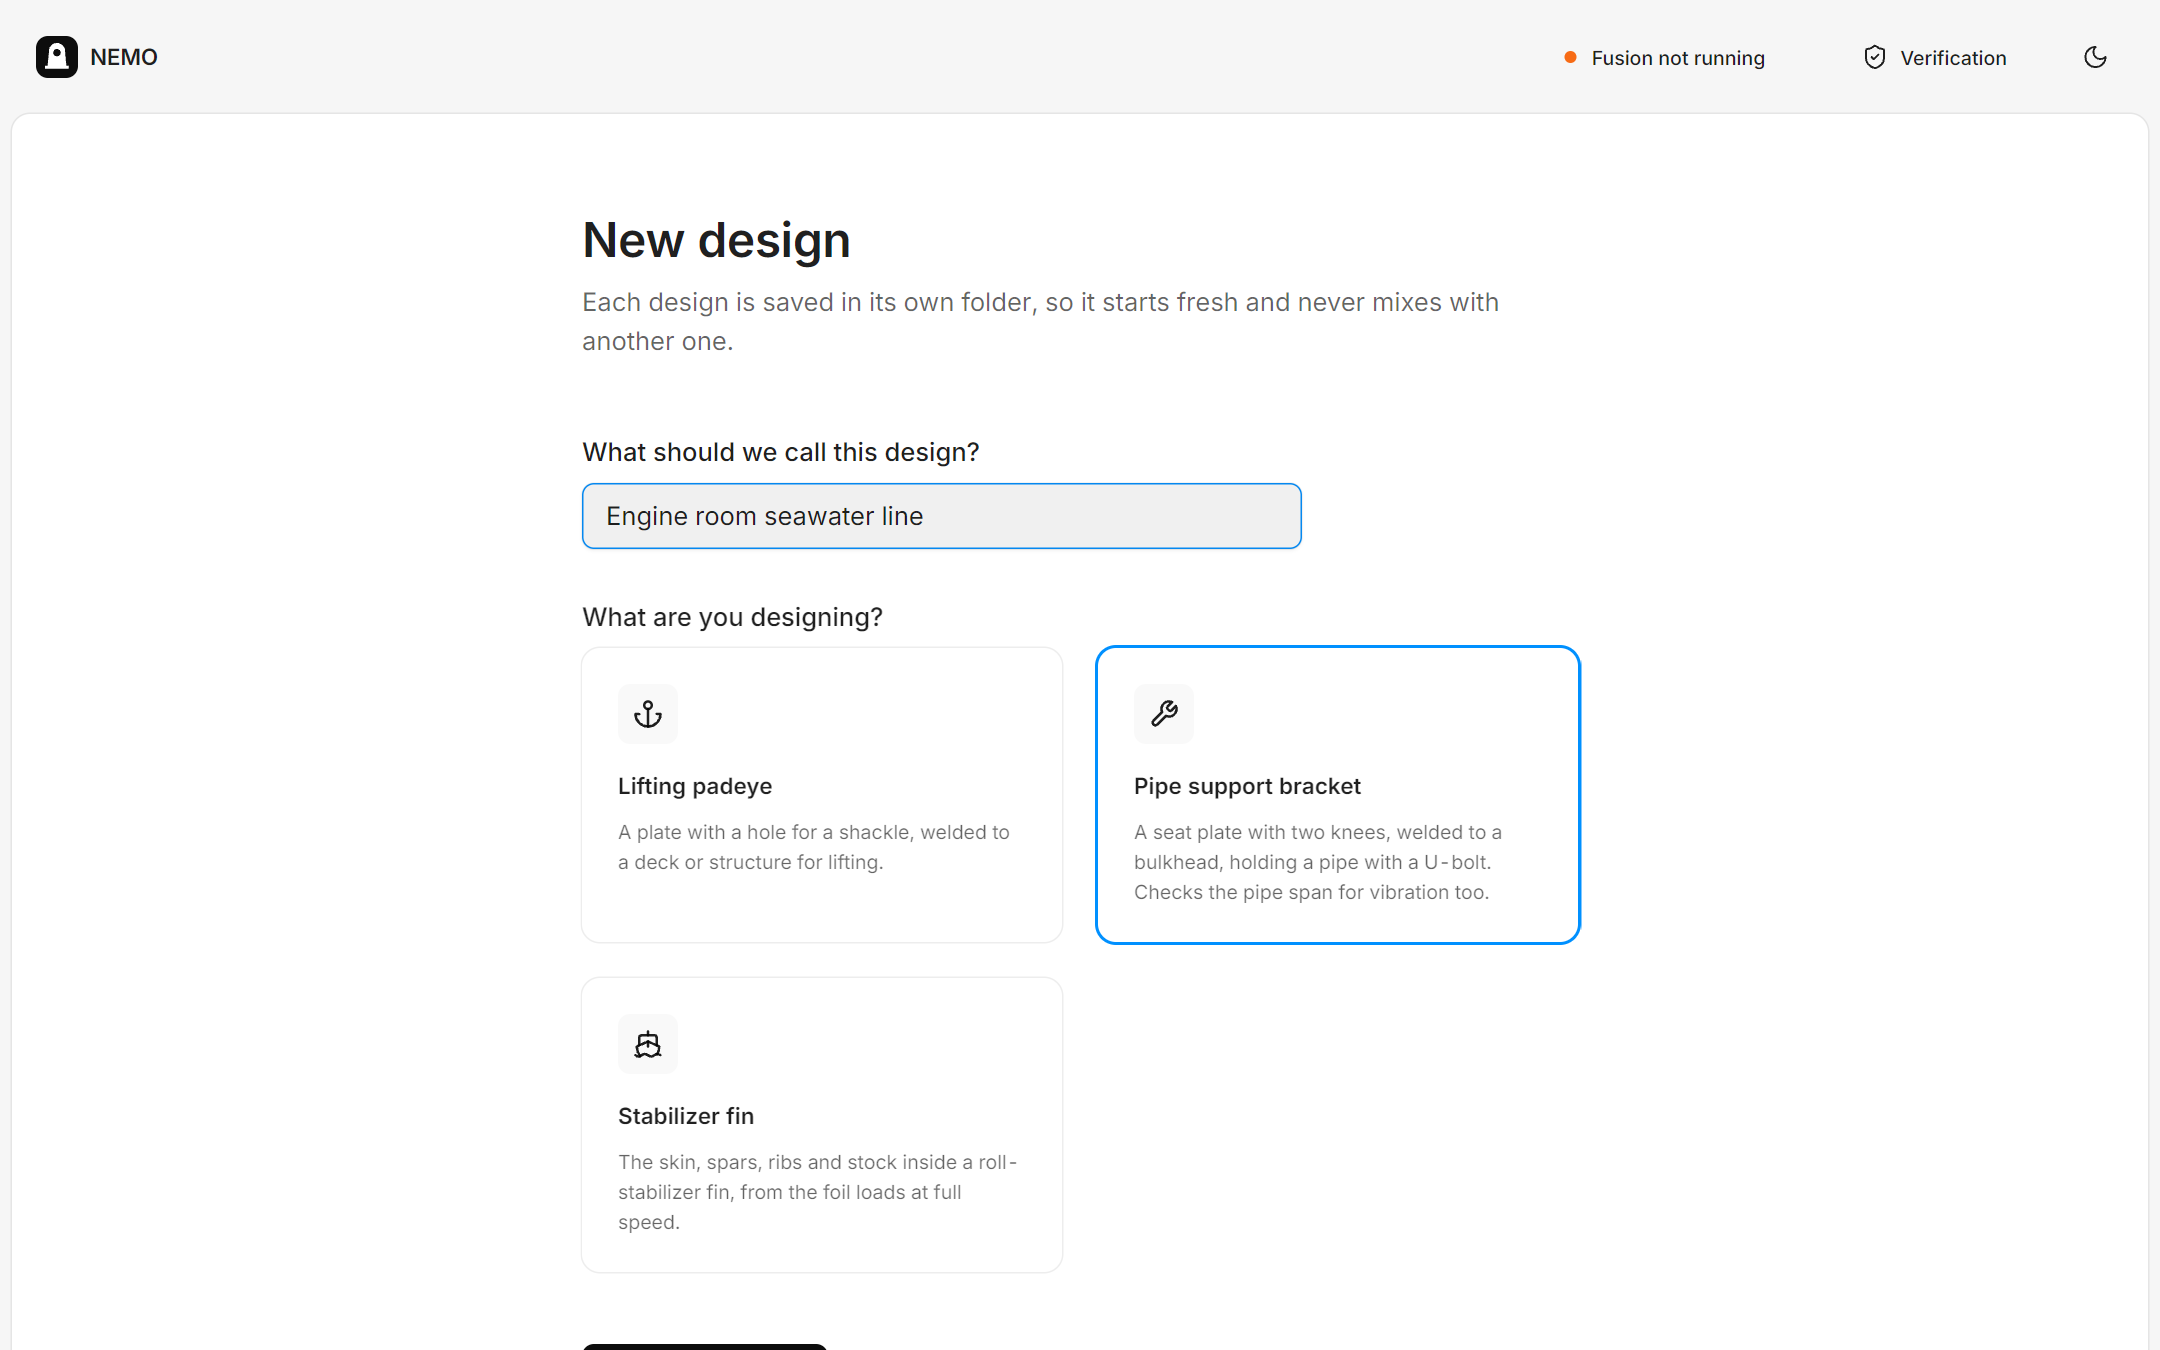
\includegraphics[width=\textwidth]{images/app-new-design.png}
\caption{Choosing the part for a new design}
\label{fig:app-new}
\end{figure}
